\section{Lab 3 - Complex Addition Systems}

\subsection{Introduction}
From your pocket calculator to inside modern CPUs adders have long been used as more than just a simple way to sum numbers together. This lab will go into the logic structure of the adder as well as provide a method for converting the simple full adder in to an \emph{arithmetic logic unit} (ALU) capable of handling 12 instructions. 

\subsection{Pre-lab}
 Truth table for half adder, full adder
Equation for a 4-bit ripple carry adder
 Block digram for a 4-bit ripple carry adder

\subsection{Lab Activities}

\subsubsection{Half Adder}
Build the circuit in Figure \ref{fig:halfadder}, create a test bench and verify that the logic is correct.

\begin{figure}[H]
	\centering
	
\includegraphics[width=60mm]{Lab3/figures/halfadder.png}
	\caption{Circuit for a 1-bit half adder}
	\label{fig:halfadder}
\end{figure}

\subsubsection{Full Adder}
The circuit in Figure \ref{fig:fulladder} implements a full 1-bit adder. Implement this circuit in VHDL, create a test bench, and verify that the logic behaves as expected. 

\begin{figure}[H]
	\centering
	
\includegraphics[width=80mm]{Lab3/figures/fulladder.png}
	\caption{Circuit for a 1-bit full adder}
	\label{fig:fulladder}
\end{figure}

Now that you have a working 1-bit full adder, implement a 4-bit ripple carry adder that sums the binary numbers "0110" and "0101." A block diagram for the 4-bit ripple carry adder is shown in Figure \ref{fig:fourbitripple}. Verify your results by creating a test bench and simulating the circuit.

\begin{figure}[H]
	\centering
	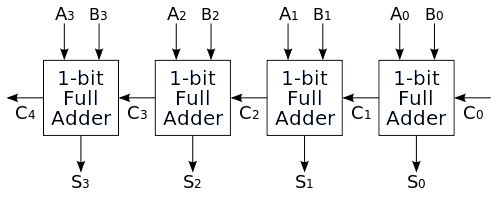
\includegraphics[width=100mm]{Lab3/figures/fourbitripple.png}
	\caption{4-bit ripple carry adder block diagram}
	\label{fig:fourbitripple}
\end{figure}

\subsubsection{Full Adder Based ALU}


\begin{tabular}{ | c | c | c | c | }
 	\hline                        
 	 Ai & Bi & D0D1 & Result \\ \hline
 	 Set to 0 & Set to 0 & 00 & 0 \\ \hline
 	 Set to 0 &  Set to 0  & 1 & 1 \\ \hline
 	 A &  Set to 0 & 0 & A \\ \hline
 	 Set to 0& B  & 0  & B  \\ \hline
 	 A & Set to 0 & 1 & A $+$ 1 \\ \hline
 	 Set to 0 & B & 1 & B $+$ 1 \\ \hline
 	 A & B & 0 & A $+$ B \\ \hline
 	 A & B & 1 & A $-$ B \\ \hline
 	 Set to invert & Set to 0 & 0 & $\overline{A}$ \\ \hline
 	 Set to invert & Set to 0 & 1 & $-$A \\ \hline
 	 Set to 0 & Set to invert & 0 &  $\overline{B}$ \\ \hline
 	 Set to 0 & Set to invert & 1 & $-$B \\
 	 \hline
\end{tabular}

\subsection{Lab Report}

%HEX0 - HEX1 - Set by SW0-7

%HEX2- HEX3 -  Set by SW8-15

%FF + FF = 1FE

%HEX4 - HEX5 = SUM

%LEDG = Overflow/carry_out

%carry_in 


%CLOCK -  KEY[0]

